%this is a test latex file
\documentclass{article}
\usepackage{CJK}
\usepackage{graphicx}
\usepackage{float}
\usepackage{indentfirst}
\usepackage{makeidx}
\usepackage{listings}% other for source code
%\usepackage{epstopdf}
%\usepackage{hyperref}
\makeindex
\lstset{language=C}
\begin{document}
\begin{CJK}{UTF8}{gbsn}
	\title {This is a test latex file}
	\author {Hanhj}
	\maketitle
	\tableofcontents
	\begin{abstract}
		这是摘要
	\end{abstract}
	\newpage
	\part{第一部分}
	\section{第1节}
        \label{mark1}
		\par
	    This is a test tex file.
		\par
		你好 \LaTeX{use tex} 
		\par 
		\begin{verbatim}
			This is test insert a code.use verbatim.
			#include <stdio.h>
			void main(){
			}
		\end{verbatim}
		\begin{lstlisting}
			This is another insert code .use listings.
			#include <stdio.h>
			void main(){}{
			
			}
		\end{lstlisting}
		This is a table test。\\
		\begin{tabular}{|l|l|l|}
			\hline
			\cline{1-3}
			a & b & c \\
			\hline
			row 1 col 1 & row 1 col 2 & row 1 col3 \\
			\hline
			row 2 col 1 & row 2 col 2 & row 2 col3 \\
			\hline
		\end{tabular}

	\section{第2节}	
		this is second section2\\
		中文,Hello。引用节\ref{mark1} 在页\pageref{mark1} 。
		\subsection{第2节第1小节}
		这是第2节的第1小节。使用行内数学公式:$\sum_a^bx_i^2$。\\
		这是行外数学公式 :$$y=x^2$$
		\par 
		这是新的一段,\index{duan}
		\newline
		这是新的一行。新的一段会首行缩进,而新的一行不会首行缩进。
	
	\part{第二部分}
	\paragraph{第1段} 使用了pargraph。与节(使用section)所不同的是不会产生数字序号
	\par
	这是一个比较长的段,(使用了par)aaaaaaaaaaaaaaaaaaaaaaaaaaaaaaaaaaaaaaaaaaa\\
	bbbbbbbbbbbbbbbbbbbbbbbbbbbbbbbbbbbbbbbbbbbbbbbbbb\\
	ccccccccccccccccccccccccc.
	\subparagraph{第一段的第一子段}  使用了subparagraph。\\
	这里使用了引用bibitem \cite{JW2}
	\par 
	插入一个eps图片\\
	\begin{figure}[H]
	\centering
	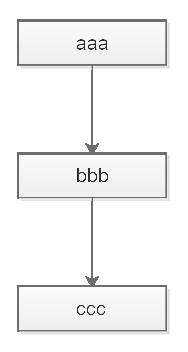
\includegraphics{test.eps}
	\caption{标题}
	\label{1}
	\end{figure}
	\index{duan}
	\begin{thebibliography}{2}
			\bibitem{JW1}引用1
			\bibitem{JW2}引用2
	\end{thebibliography}

	\printindex
\end{CJK}
\end{document}
